% Template for Cogsci submission with R Markdown

% Stuff changed from original Markdown PLOS Template
\documentclass[10pt, letterpaper]{article}

\usepackage{cogsci}
\usepackage{pslatex}
\usepackage{float}
\usepackage{caption}

% amsmath package, useful for mathematical formulas
\usepackage{amsmath}

% amssymb package, useful for mathematical symbols
\usepackage{amssymb}

% hyperref package, useful for hyperlinks
\usepackage{hyperref}

% graphicx package, useful for including eps and pdf graphics
% include graphics with the command \includegraphics
\usepackage{graphicx}

% Sweave(-like)
\usepackage{fancyvrb}
\DefineVerbatimEnvironment{Sinput}{Verbatim}{fontshape=sl}
\DefineVerbatimEnvironment{Soutput}{Verbatim}{}
\DefineVerbatimEnvironment{Scode}{Verbatim}{fontshape=sl}
\newenvironment{Schunk}{}{}
\DefineVerbatimEnvironment{Code}{Verbatim}{}
\DefineVerbatimEnvironment{CodeInput}{Verbatim}{fontshape=sl}
\DefineVerbatimEnvironment{CodeOutput}{Verbatim}{}
\newenvironment{CodeChunk}{}{}

% cite package, to clean up citations in the main text. Do not remove.
\usepackage{apacite}

% KM added 1/4/18 to allow control of blind submission
\cogscifinalcopy

\usepackage{color}

% Use doublespacing - comment out for single spacing
%\usepackage{setspace}
%\doublespacing


% % Text layout
% \topmargin 0.0cm
% \oddsidemargin 0.5cm
% \evensidemargin 0.5cm
% \textwidth 16cm
% \textheight 21cm

\title{Peekbank: Exploring children's word recognition through an open,
large-scale repository for developmental eye-tracking data}

\usepackage[raggedright]{sidecap}

\author{{\large \bf Martin Zettersten (martincz@princeton.edu)\textsuperscript{1}}, {\large \bf Claire Bergey\textsuperscript{2}}, {\large \bf Naiti S. Bhatt\textsuperscript{3}}, {\large \bf Veronica Boyce\textsuperscript{4}},  \\ {\large \bf Mika Braginsky\textsuperscript{5}}, {\large \bf Alexandra Carstensen\textsuperscript{4}}, {\large \bf Benny deMayo\textsuperscript{1}}, {\large \bf George Kachergis\textsuperscript{4}},  \\ {\large \bf Molly Lewis\textsuperscript{6}}, {\large \bf Bria Long\textsuperscript{4}}, {\large \bf Kyle MacDonald\textsuperscript{7}}, {\large \bf Jessica Mankewitz\textsuperscript{4}},  \\ {\large \bf Stephan Meylan\textsuperscript{5,8}}, {\large \bf Annissa N. Saleh\textsuperscript{9}}, {\large \bf Rose M. Schneider\textsuperscript{10}}, {\large \bf Angeline Sin Mei Tsui\textsuperscript{4}},  \\ {\large \bf Sarp Uner\textsuperscript{8}}, {\large \bf Tian Linger Xu\textsuperscript{11}}, {\large \bf Daniel Yurovsky\textsuperscript{6}}, {\large \bf Michael C. Frank (mcfrank@stanford.edu)\textsuperscript{4}}  \\ {\textsuperscript{1}}Dept. of Psychology, Princeton University, {\textsuperscript{2}}Dept. of Psychology, University of Chicago,  \\ {\textsuperscript{3}}Scripps College, {\textsuperscript{4}}Dept. of Psychology, Stanford University, {\textsuperscript{5}}Dept. of Brain and Cognitive Sciences, MIT,  \\ {\textsuperscript{6}}Dept. of Psychology, Carnegie Mellon University, {\textsuperscript{7}}Core Technology, McD Tech Labs,  \\ {\textsuperscript{8}}Dept. of Psychology and Neuroscience, Duke University, {\textsuperscript{9}}Dept. of Psychology, UT Austin \\ {\textsuperscript{10}}Dept. of Psychology, UC San Diego, {\textsuperscript{11}}Dept. of Psychological and Brain Sciences, Indiana University}


\begin{document}

\maketitle

\begin{abstract}
The ability to rapidly recognize words and link them to referents in
context is central to children's early language development. This
ability, often called word recognition in the developmental literature,
is typically studied in the looking-while-listening paradigm, which
measures infants' fixation on a target object (vs.~a distractor) after
hearing a target label. We present a large-scale, open database of
infant and toddler eye-tracking data from looking-while-listening tasks.
The goal of this effort is to address theoretical and methodological
challenges in measuring vocabulary development. We present two analyses
of the current database (\emph{N}=1,320): (1) capturing age-related
changes in infants' word recognition while generalizing across
item-level variability and (2) assessing how a central methodological
decision -- selecting the time window of analysis -- impacts the
reliability of measurement. Future efforts will expand the scope of the
current database to advance our understanding of participant-level and
item-level variation in children's vocabulary development.

\textbf{Keywords:}
word recognition; eye-tracking; vocabulary development;
looking-while-listening
\end{abstract}

\hypertarget{introduction}{%
\section{Introduction}\label{introduction}}

Across their first years of life, children learn words in their native
tongues at a rapid pace (Frank, Braginsky, Yurovsky, \& Marchman, 2021).
A key facet of children's growing word knowledge is their ability to
efficiently process words and link them to relevant meanings -- often
termed word recognition. Developing word recognition skills builds a
foundation for language development; for example, the speed and accuracy
with which infants process words are predictive of later linguistic and
cognitive outcomes (e.g., Marchman et al., 2018).

Word recognition is traditionally studied in the
``looking-while-listening'' paradigm (or alternatively in a version of
the intermodal preferential looking paradigm; Fernald, Zangl, Portillo,
\& Marchman, 2008; Hirsh-Pasek, Cauley, Golinkoff, \& Gordon, 1987). In
such studies, infants listen to a sentence prompting a specific referent
(e.g., \emph{Look at the dog!}) while viewing two images on the screen
(e.g., an image of a dog -- the target image -- and an image of a duck
-- the distractor image). Infants' word recognition is measured in terms
of how quickly and accurately they fixate on the correct target image
after hearing its label. Studies using this design have contributed to
our understanding of a wide range of questions in language development,
including infants' early noun knowledge, phonological representations of
words, prediction during language processing, and individual differences
in language development (Bergelson \& Swingley, 2012; Golinkoff, Ma,
Song, \& Hirsh-Pasek, 2013; Lew-Williams \& Fernald, 2007; Marchman et
al., 2018; Swingley \& Aslin, 2000).

While the looking-while-listening paradigm has been highly fruitful in
advancing understanding of early word knowledge, fundamental questions
remain both about the trajectory of children's word recognition ability
and how to improve measurement of children's word recognition in the
first place. One central question is how to measure developmental change
in the speed and accuracy of word recognition. In language development
research, processing speed - the ability to quickly link a word to its
referent - has been of key interest because it is thought to both
reflect past language learning and to support subsequent learning.
Age-related changes in speed of processing are argued to accelerate
infants' learning: as infants begin to process incoming speech input
faster, they become better equipped to learn from their language
environment (Fernald \& Marchman, 2012). Consistent with this
hypothesis, longitudinal analyses have found that individual differences
in word recognition speed predict linguistic and cognitive outcomes
later in childhood (e.g., Marchman \& Fernald, 2008). However, measuring
increases in the speed and accuracy of word recognition faces the
challenge of distinguishing developmental changes in word recognition
skill from changes in knowledge of specific words. This problem is
particularly thorny in child development research, since the number of
items that can be tested within a single session is limited and items
must be selected in an age-appropriate manner (Peter et al., 2019). One
way to overcome this challenge is to measure word recognition across
development in a large-scale dataset with a wide range of items. A
sufficiently large dataset would allow researchers to estimate
developmental change in word recognition speed and accuracy while
generalizing across changes related to specific words.

A second question relates to evaluating methodological best practices.
In particular, many fundamental analytic decisions vary substantially
across studies, and different decisions may lead to different inferences
about children's word recognition. For example, researchers vary in how
they select time windows for analysis, transform the dependent measure
of target fixations, and model the time course of word recognition
(Csibra, Hernik, Mascaro, Tatone, \& Lengyel, 2016; Fernald et al.,
2008; Huang \& Snedeker, 2020). This problem is made more complex by the
fact that many of these decisions depend on a variety of design-related
and participant-related factors (e.g., infant age). Establishing best
practices therefore requires a large database of infant word recognition
studies varying across such factors, in order to test the potential
consequences of methodological decisions on study results.

What these two questions share is that they are difficult to answer at
the scale of a single study. To address this challenge, we introduce
\emph{Peekbank} (\url{https://peekbank.stanford.edu/}), a flexible and
reproducible interface to an open database of developmental eye-tracking
studies. The Peekbank project (a) collects a large set of eye-tracking
datasets on children's word recognition, (b) introduces a data format
and tools for standardizing eye-tracking data across data sources, and
(c) provides an interface for accessing and analyzing the database. In
creating the Peekbank database, the project pursues two main aims: to
answer central theoretical questions about lexical development and to
provide data-driven guidance on methodological decisions. In the current
paper, we give an overview of the key components of the project and
demonstrate its utility in advancing theoretical and methodological
insights. We report two analyses using the database and associated tools
(\emph{N}=1,320): (1) a growth curve analysis modeling age-related
changes in infants' word recognition while generalizing across
item-level variability; and (2) a multiverse-style analysis of how a
central methodological decision -- selecting the time window of analysis
-- impacts inter-item reliability.

\hypertarget{methods}{%
\section{Methods}\label{methods}}

\begin{table*}[ht]
\centering
\begingroup\fontsize{9pt}{10pt}\selectfont
\begin{tabular}{lrrrrrr}
  \hline
Dataset Name & Citation & N & Mean Age (mos.) & Age Range (mos.) & Method & Language \\ 
  \hline
attword & (Yurovsky \& Frank, 2017) & 288 & 25.5 & 13 - 59 & eye-tracking & English \\ 
  canine & unpublished & 36 & 23.8 & 21 - 27 & manual coding & English \\ 
  coartic & (Mahr et al., 2015) & 29 & 20.8 & 18 - 24 & eye-tracking & English \\ 
  cowpig & (Perry et al., 2017) & 45 & 20.5 & 19 - 22 & manual coding & English \\ 
  ft\_pt & (Adams et al., 2018) & 69 & 17.1 & 13 - 20 & manual coding & English \\ 
  mispron & (Swingley \& Aslin, 2002) & 50 & 15.1 & 14 - 16 & manual coding & English \\ 
  mix & (Byers-Heinlein et al., 2017) & 48 & 20.1 & 19 - 21 & eye-tracking & English, French \\ 
  reflook\_socword & (Yurovsky et al., 2013) & 435 & 33.6 & 12 - 70 & eye-tracking & English \\ 
  reflook\_v4 & unpublished & 45 & 34.2 & 11 - 60 & eye-tracking & English \\ 
  remix & (Potter et al., 2019) & 44 & 22.6 & 18 - 29 & manual coding & Spanish, English \\ 
  salientme & (Pomper \& Saffran, 2019) & 44 & 40.1 & 38 - 43 & manual coding & English \\ 
  switchingCues & (Pomper \& Saffran, 2016) & 60 & 44.3 & 41 - 47 & manual coding & English \\ 
  tablet & (Frank et al., 2016) & 69 & 35.5 & 12 - 60 & eye-tracking & English \\ 
  tseltal & (Casillas et al., 2017) & 23 & 31.3 & 9 - 48 & manual coding & Tseltal \\ 
  yoursmy & (Garrison et al., 2020) & 35 & 14.5 & 12 - 18 & eye-tracking & English \\ 
   \hline
\end{tabular}
\endgroup
\caption{Overview over the datasets in the current database.} 
\end{table*}

\hypertarget{database-framework}{%
\subsection{Database Framework}\label{database-framework}}

\begin{CodeChunk}
\begin{figure}[tb]

{\centering 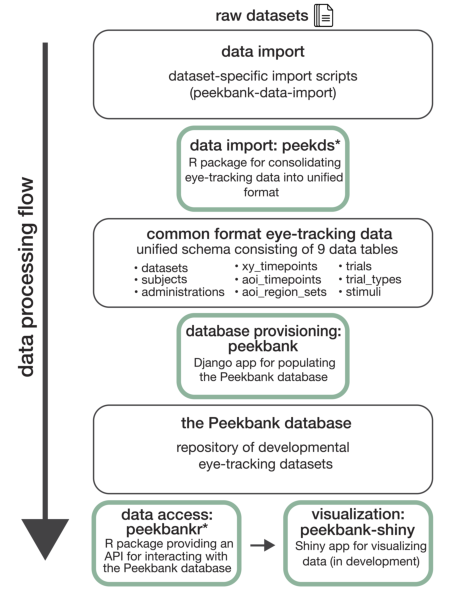
\includegraphics{figs/fig_framework_overview-1} 

}

\caption[Overview of the Peekbank data ecosystem]{Overview of the Peekbank data ecosystem. Peekbank tools are highlighted in green. *custom R packages.}\label{fig:fig_framework_overview}
\end{figure}
\end{CodeChunk}

The Peekbank data framework consists of three components: (1) processing
raw experimental datasets; (2) populating a relational database; and (3)
providing an interface to the database (Fig.
\ref{fig:fig_framework_overview}). The \texttt{peekds} library (for the
R language; R Development Core Team, 2020) helps researchers convert and
validate existing datasets to use the relational format of the database.
The \texttt{peekbank} module (Python) creates a database with the
relational schema and populates it with the standardized datasets
produced by \texttt{peekds}. The database is implemented in MySQL, an
industry standard relational database, which may be accessed by a
variety of programming languages over the internet. The
\texttt{peekbankr} library (R) provides an application programming
interface, or API, that offers high-level abstractions for accessing
data in Peekbank.

\hypertarget{data-format-and-processing}{%
\subsection{Data Format and
Processing}\label{data-format-and-processing}}

One of the main challenges in compiling a large-scale eye-tracking
dataset is the lack of a shared re-usable data format across individual
experiments. Researcher conventions for structuring data vary, as do the
technical specifications of different devices, rendering the task of
integrating datasets from different labs and data sources difficult. We
developed a common, tidy format for the eye-tracking data in Peekbank to
ease the process of conducting cross-dataset analyses (Wickham et al.,
2019). The schema of the database is sufficiently general to handle
heterogeneous datasets, including both manually coded and automated
eye-tracking data.

During data import, raw eye-tracking datasets are processed to conform
to the Peekbank data schema. The centerpiece of the schema is the
\texttt{aoi\textunderscore timepoints} table (Fig.
\ref{fig:fig_framework_overview}), which records whether participants
looked to the target or the distractor stimulus at each timepoint of a
given trial. Additional tables track information about data sources,
participants, trials, stimuli, and raw eye-tracking data. In addition to
unifying the data format, we conduct several pre-processing steps to
facilitate analyses across datasets. First, we normalize time relative
to the onset of the target label, since the main goal is to assess
participants' fixation of the target image in response to hearing its
corresponding label. Second, we resample observations to a common
sampling rate (40 Hz), in order to ease data visualization and analysis.
Where necessary (e.g., if the original data was sampled at 30 Hz),
observations are interpolated by selecting the gaze location at the
nearest time point in the original data.

\hypertarget{current-data-sources}{%
\subsection{Current Data Sources}\label{current-data-sources}}

The database currently includes 15 looking-while-listening datasets
comprising \emph{N}=1320 total participants (Table 1). Most datasets (12
out of 15 total) consist of data from monolingual native English
speakers. They span a wide age spectrum with participants ranging from 9
to 70 months of age, and are balanced in terms of gender (46\% female).
The datasets vary across a number of design-related dimensions, and
include studies using manually coded video recordings and automated
eye-tracking methods (e.g., Tobii, EyeLink) to measure gaze behavior.
All studies tested familiar items, but the database also includes 5
datasets that tested novel pseudo-words in addition to familiar words.
All data are openly available on the Open Science Framework
(\url{https://osf.io/pr6wu/}).

\sidecaptionvpos{figure}{c}
\begin{SCfigure*}[0.2] 
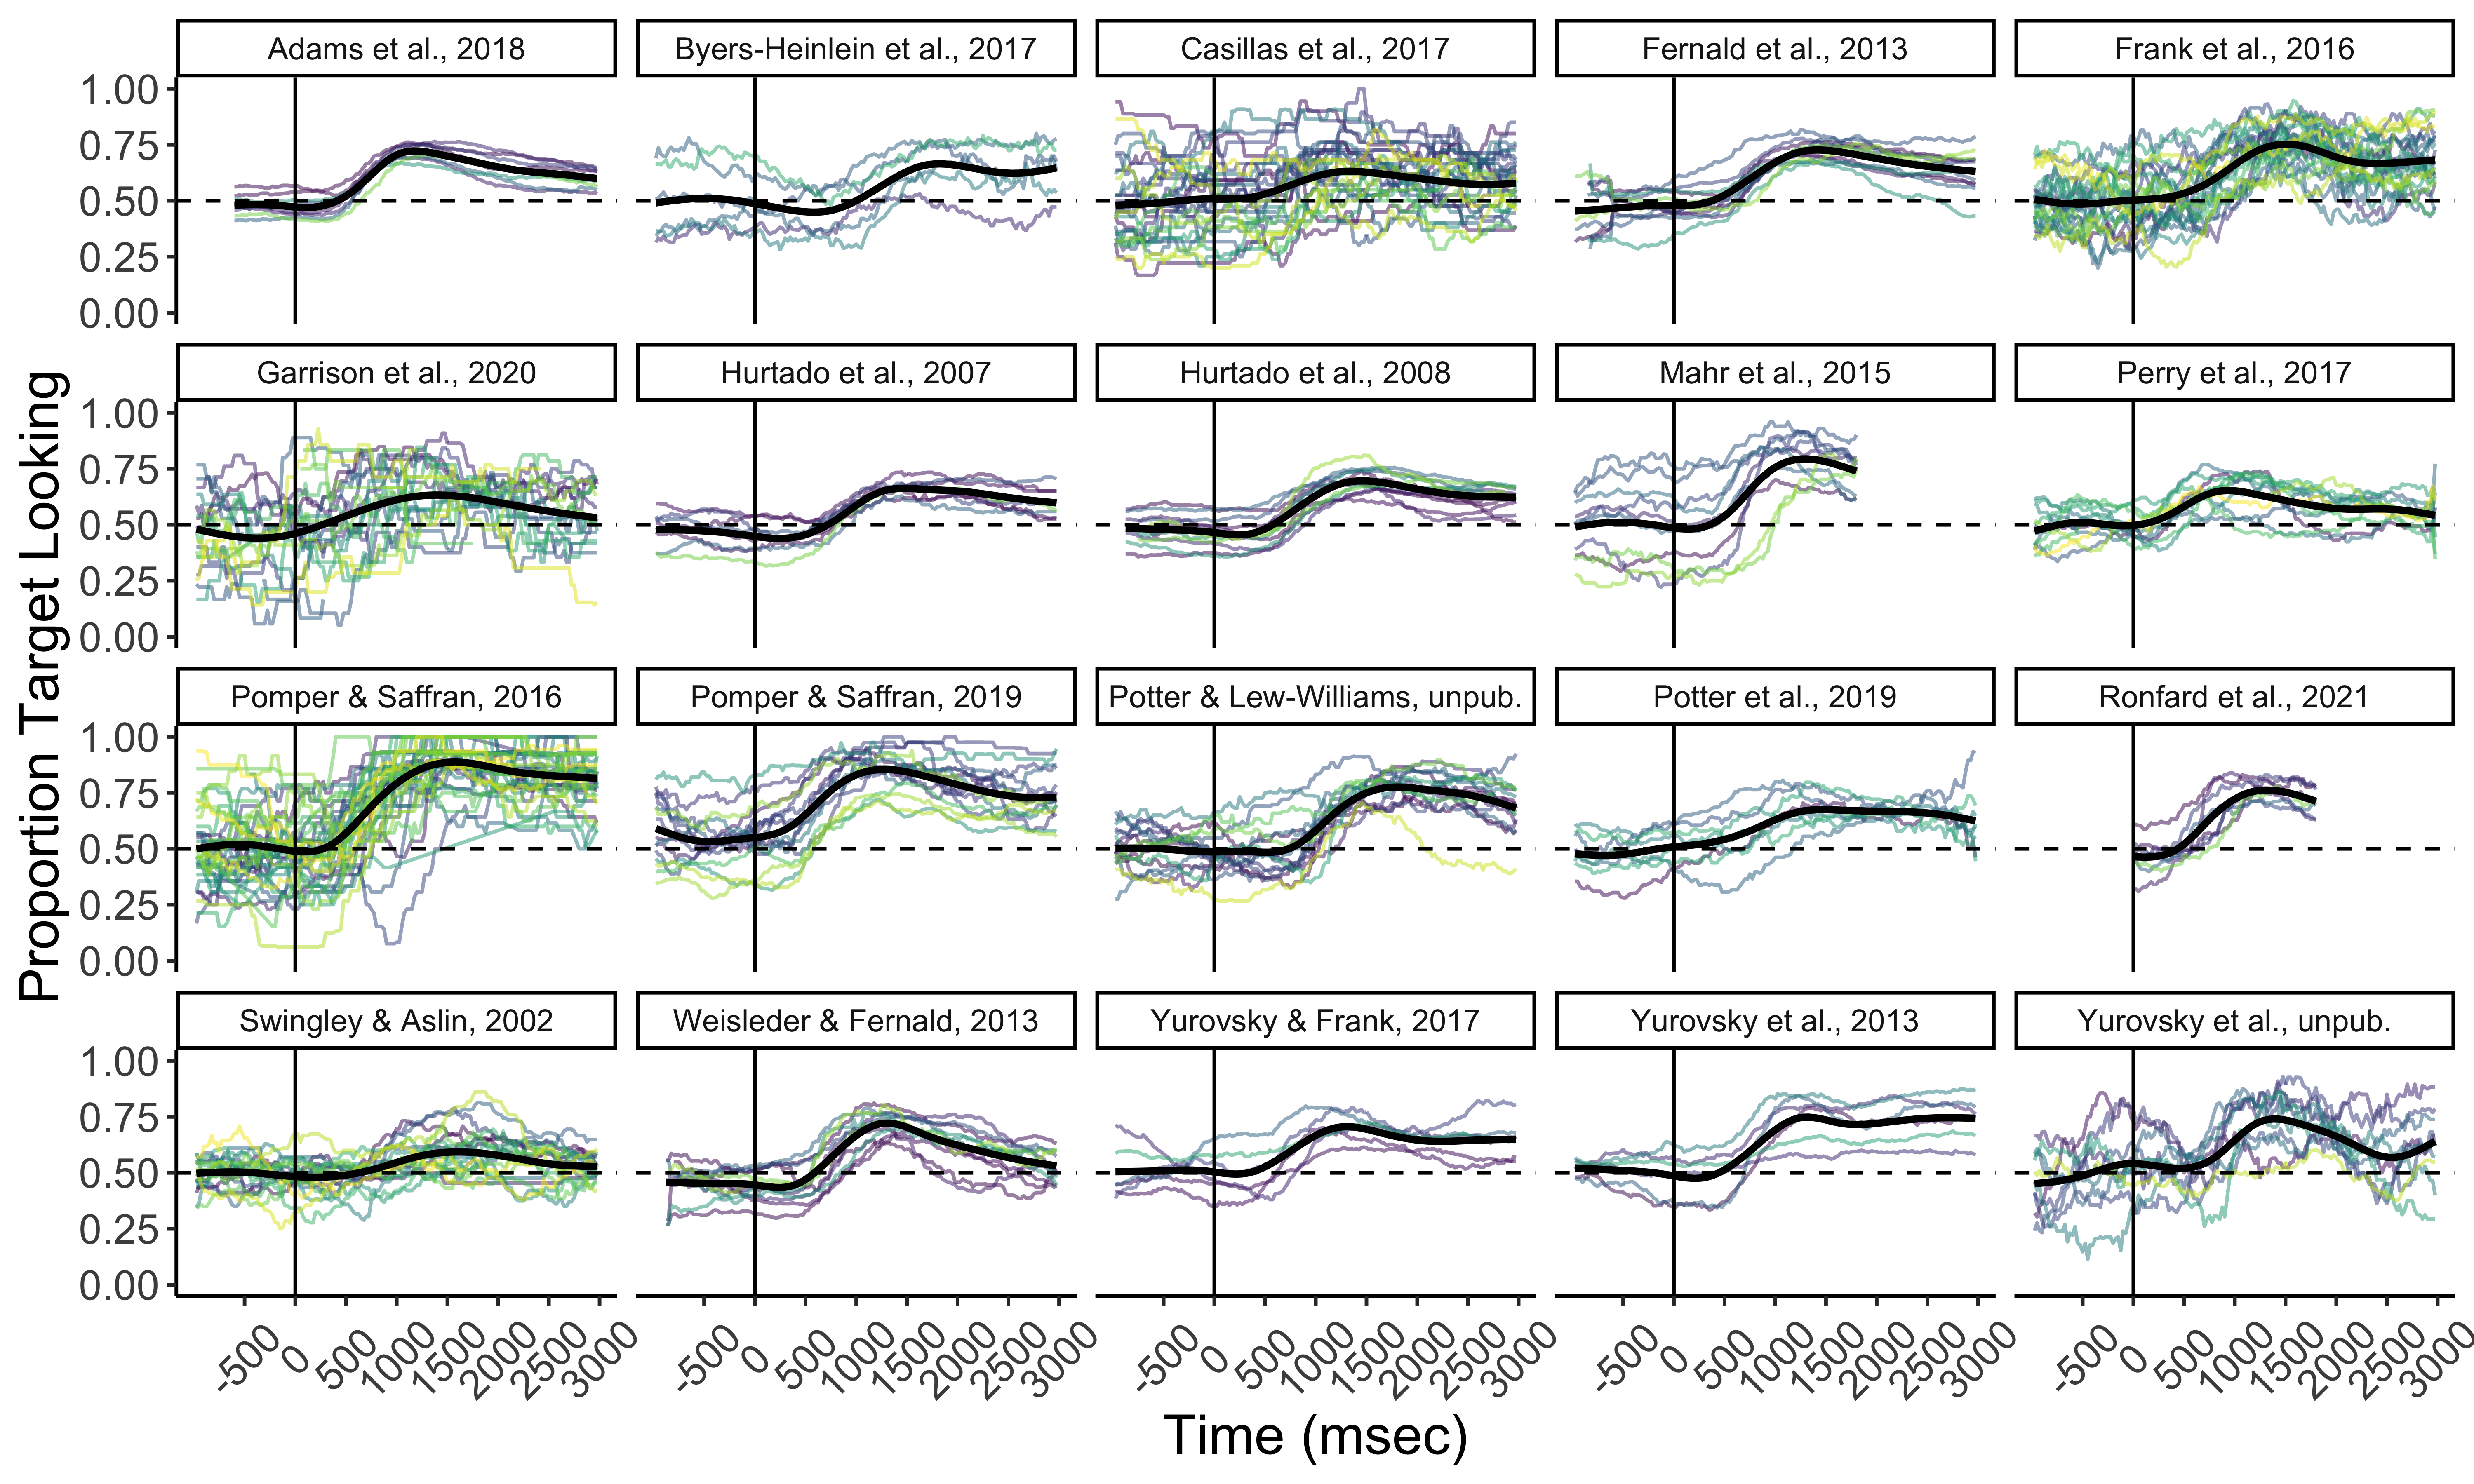
\includegraphics[width=14cm,height=8.4cm]{../figures/peekbank_item_vis.png}
\caption{Item-level variability in proportion target looking within each dataset (chance=0.5). Time is centered on the onset of the target label (vertical line). Colored lines represent specific target labels. Black lines represent smoothed average fits based on a general additive model using cubic splines. See Table 1 for details on each dataset.}
\label{fig:peekbank_item_vis}
\end{SCfigure*}

\hypertarget{results}{%
\section{Results}\label{results}}

\hypertarget{general-descriptives-and-item-variability}{%
\subsection{General descriptives and Item
Variability}\label{general-descriptives-and-item-variability}}

\begin{table}[H]
\centering
\begingroup\fontsize{9pt}{10pt}\selectfont
\begin{tabular}{lrrl}
  \hline
Dataset Name & Unique Items & Prop. Target & 95\% CI \\ 
  \hline
attword & 6 & 0.63 & [0.61, 0.64] \\ 
  canine & 16 & 0.64 & [0.61, 0.67] \\ 
  coartic & 10 & 0.70 & [0.67, 0.73] \\ 
  cowpig & 12 & 0.60 & [0.58, 0.63] \\ 
  ft\_pt & 8 & 0.64 & [0.63, 0.66] \\ 
  mispron & 22 & 0.57 & [0.55, 0.59] \\ 
  mix & 6 & 0.55 & [0.52, 0.58] \\ 
  reflook\_socword & 6 & 0.61 & [0.6, 0.63] \\ 
  reflook\_v4 & 10 & 0.61 & [0.57, 0.65] \\ 
  remix & 8 & 0.62 & [0.58, 0.66] \\ 
  salientme & 16 & 0.73 & [0.71, 0.75] \\ 
  switchingCues & 40 & 0.77 & [0.75, 0.79] \\ 
  tablet & 24 & 0.63 & [0.6, 0.67] \\ 
  tseltal & 30 & 0.59 & [0.54, 0.63] \\ 
  yoursmy & 87 & 0.60 & [0.56, 0.64] \\ 
   \hline
\end{tabular}
\endgroup
\caption{Average proportion target looking in each dataset.} 
\end{table}

Analysis scripts for all results are openly available at
\url{https://github.com/langcog/peekbank-paper}. In general,
participants demonstrated robust, above-chance word recognition in each
dataset (chance=0.5). Table 2 shows the average proportion of target
looking within a standard critical window of 300-2000ms after the onset
of the label for each dataset (Swingley \& Aslin, 2000). The number of
unique target labels and their associated accuracy vary widely across
datasets (Figure \ref{fig:peekbank_item_vis}). Proportion target looking
was generally higher for familiar words (\emph{M} = 0.66, 95\% CI =
{[}0.65, 0.67{]}, \emph{n} = 1269) than for novel words learned during
the experiment (\emph{M} = 0.59, 95\% CI = {[}0.58, 0.61{]}, \emph{n} =
822).

\hypertarget{predicting-age-related-changes-while-generalizing-across-items}{%
\subsection{Predicting Age-Related Changes While Generalizing Across
Items}\label{predicting-age-related-changes-while-generalizing-across-items}}

Developmental changes in word recognition have been a central issue
since early investigations of eye-tracking techniques (Fernald, Pinto,
Swingley, Weinberg, \& McRoberts, 1998). Children's speed and accuracy
of word recognition increases across early childhood, yet measuring
these increases presents an item selection puzzle for researchers: Words
that are appropriate for an 18-month-old will be too easy for a
three-year-old; those that are appropriate for a three-year-old will be
difficult for the 18-month-old. Failure to choose appropriate test items
can even lead to spurious conclusions about development (Peter et al.,
2019).

This issue is familiar in psychometrics: test developers interested in
measuring across a wide range of a particular latent ability must choose
items appropriate for different abilities. One solution is to use data
from a bank of questions that have been taken by test-takers of a range
of abilities, and then use item-response theory models to create
different test versions appropriate for different ability ranges
(Embretson \& Reise, 2000). Such tests can then be used to extract
estimates of developmental change that are independent of individual
tests and their particular items.

Peekbank provides the appropriate large-scale database for estimating
these item-independent developmental changes and designing
age-appropriate tests in the future. Here we show a proof of concept by
providing an estimate of the item-independent growth of word recognition
accuracy across development. We take advantage of the equivalence
between item response theory and linear mixed-effects models (LMMs; De
Boeck et al., 2011), using LMMs to model the trajectory of word
recognition across age. We follow the approach of Mirman (2014) and use
growth curve LMMs to predict the time course of recognition.
Specifically, we predicted children's proportion of target looking
during an early window of time (0-1500ms, chosen to avoid modeling
declines in looking later in the trial), using an empirical logit
transform on the proportion of target looking to allow the use of linear
(rather than logistic) regression models. We focused our analysis on
familiar words and included only datasets testing infants with
monolingual English language exposure (12 datasets, see Table 1). Our
predictors were time after word onset and age, and we additionally
included polynomial functions of time (up to fourth order) and quadratic
effects of age, as well as their interactions. We subtracted all
intercepts to force fits to start at a baseline of 0 (chance
performance) at time zero. As a random effect structure, we included
by-item, by-subject, and by-dataset random intercepts; though larger
random effect structures could be justified by the data, the size of the
dataset precluded fitting these. The random effect structure allows us
to model word recognition while generalizing across items and
participants.

Figure \ref{fig:age_gca} depicts the results of this analysis. Panel A
shows the mean empirical word recognition curves for four age groups,
along with fitted model performance. Although model fits are acceptable,
developmental change appears irregular -- for example, 12- to
24-month-olds show slightly earlier recognition than 24- to
36-month-olds. This pattern is likely an artifact of averaging across
datasets with substantially different items. Panel B shows model
predictions for the population level of each random effect -- our best
estimates of the latent ability structure. Here we see continuous
increases in both speed (point at which the curve rises) and accuracy
(asymptote of the curve) across ages, though this developmental trend
decelerates (consistent with other work on reaction time development;
Frank, Lewis, \& MacDonald, 2016; Kail, 1991). This proof of concept
suggests that Peekbank can be used to model developmental change over
multiple years, overcoming the limitations of individual datasets.

\sidecaptionvpos{figure}{c}
\begin{SCfigure*}[0.2] 
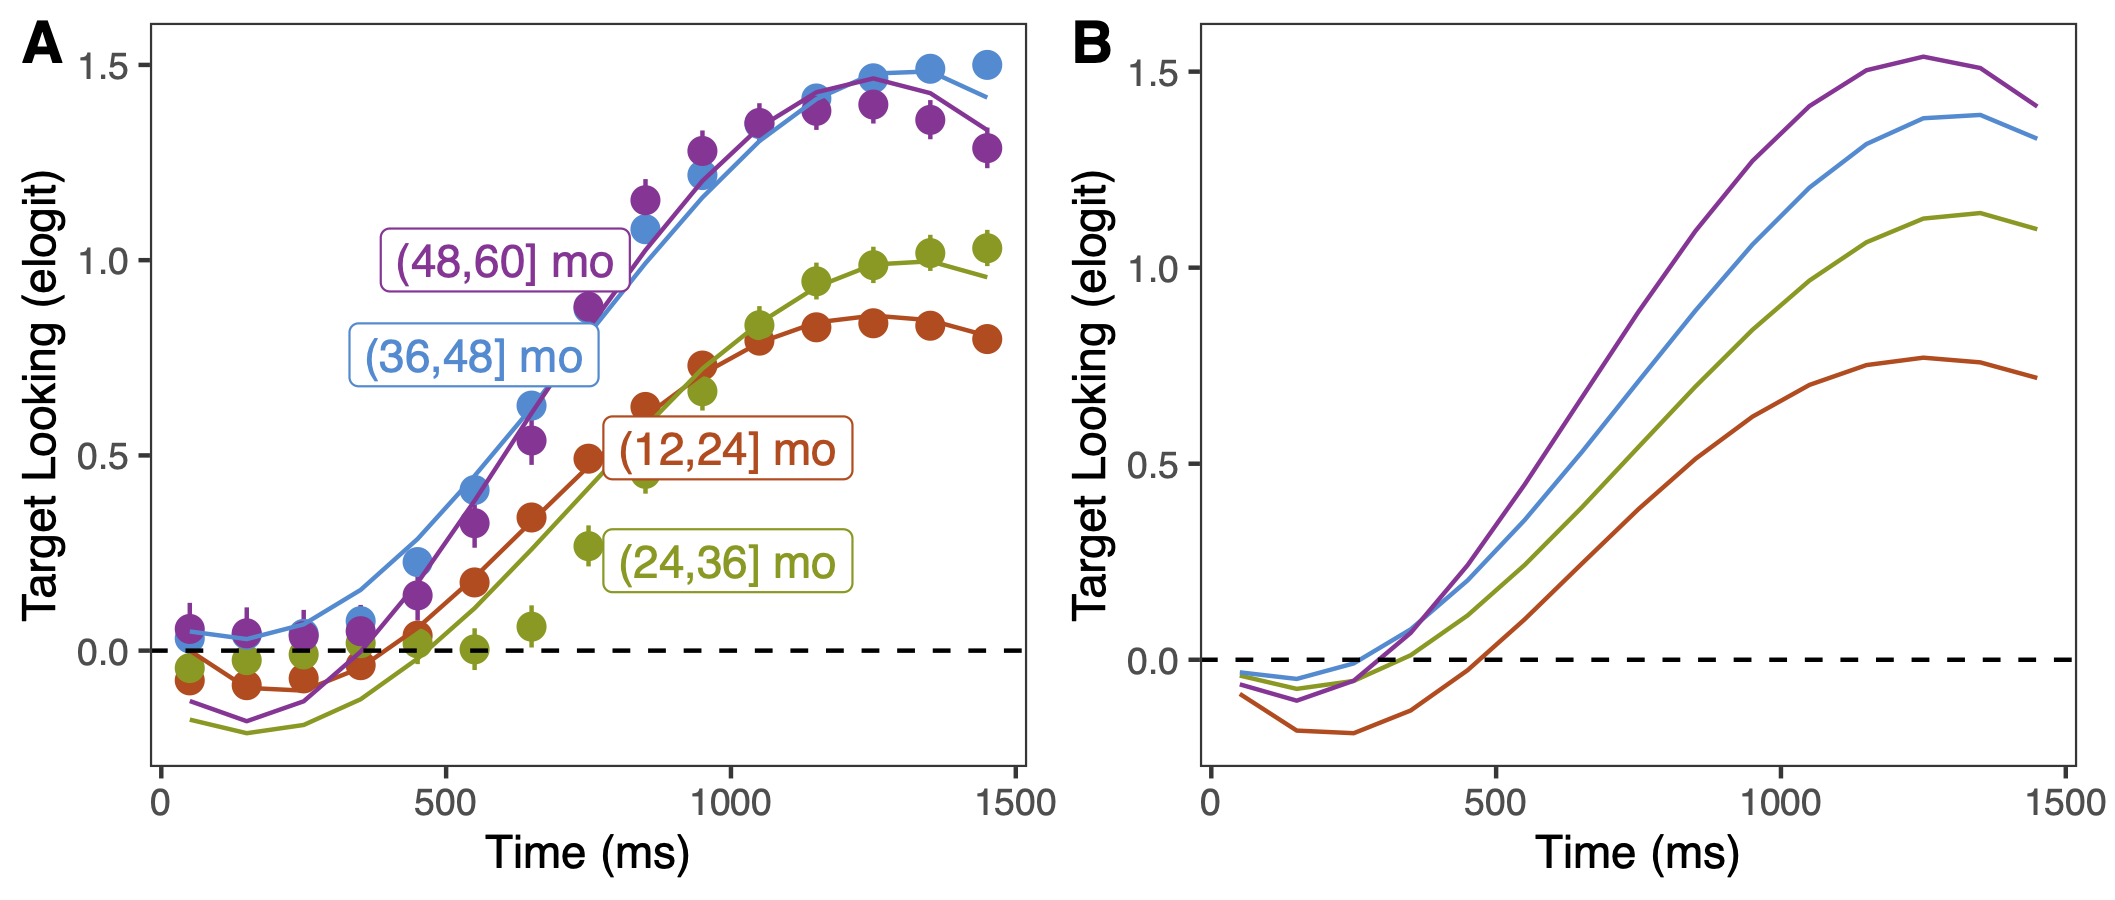
\includegraphics[width=14cm,height=6cm]{../figures/age_gca.png}
\caption{Growth curve models of proportion target looking during the critical target window at each age range (in months). (A) Mean empirical word recognition fit. (B) Population-level estimates.}
\label{fig:age_gca}
\end{SCfigure*}

\hypertarget{time-window-selection}{%
\subsection{Time Window Selection}\label{time-window-selection}}

In our second analysis, we address an analytic decision researchers
often face: how to summarize time course data into a single measure of
accuracy. Taking a similar approach to that of Peelle \& Van Engen
(2020), we conducted a multiverse-style analysis considering possible
time windows researchers might select (Steegen, Tuerlinckx, Gelman, \&
Vanpaemel, 2016). Our multiverse analysis focuses on the reliability of
participants' response to familiar words by measuring the subject-level
inter-item correlation (IIC) for proportion of looking at familiar
targets. The time windows selected by researchers vary substantially in
the literature, with some studies analyzing shorter time windows between
300ms and 1800-2000ms post-target onset (Fernald et al., 2008; Swingley
\& Aslin, 2000), and others using longer time windows extending to
approximately 3000-4000ms (especially with younger infants; e.g.,
Bergelson \& Swingley, 2012). We thus examined a broad range of window
start times ranging from 300ms pre-target onset to 1500ms post-target
onset and window end times ranging from 0ms to 4000ms post-target onset.
For each combination of window start time and end time with a minimum
window duration of 50ms, we calculated participants' average inter-item
correlation for proportion of looking at familiar targets (mean IIC)
within each dataset and subsequently averaged inter-item correlations
across datasets. Since observations were unevenly distributed across the
age range, and because children likely show a varying response to
familiar items as they age (often motivating different window choices),
we split our data into four age bins (12-24, 24-36, 36-48, and 48-60
months). We restricted the analysis within a given age bin to include
only datasets that contributed at least 5 unique test sessions. While it
is an open question what space of possible windows will yield the
greatest reliability, we expect to see low reliability (i.e.~0) in
windows that start before target onset and in windows that end within
300ms post-target onset, before participants can execute a response.

Results from this multiverse analysis are shown in Figure
\ref{fig:time_window}, where each colored pixel represents the mean IIC
for proportion of looking to familiar targets for a specific combination
of window start and end time. The analysis shows that IIC is positive
(red) under a wide range of sensible window choices. IIC is relatively
low however, especially for the youngest age group, suggesting that
individual items carry only limited shared signal regarding children's
underlying ability.

Intriguingly, however, late end times and long overall window lengths
tend to show higher reliability than shorter windows. Shorter windows
(e.g., 300-2000ms, as we used above) likely maximize absolute
recognition performance by fitting the peak of the recognition curve,
but simultaneously may lower reliability by failing to include all
relevant data. Especially for older children, higher IICs tended to be
found with windows that started between 300 and 1000ms and ended between
2500 and 4000ms. This finding is sensible from a psychometric
perspective -- averaging more timepoints (even if some contain limited
signal) increases reliability and reduces variation. Thus, researchers
interested in better measurement of individual variation or condition
differences could consider using longer windows by default.

\begin{SCfigure*}[0.25] 
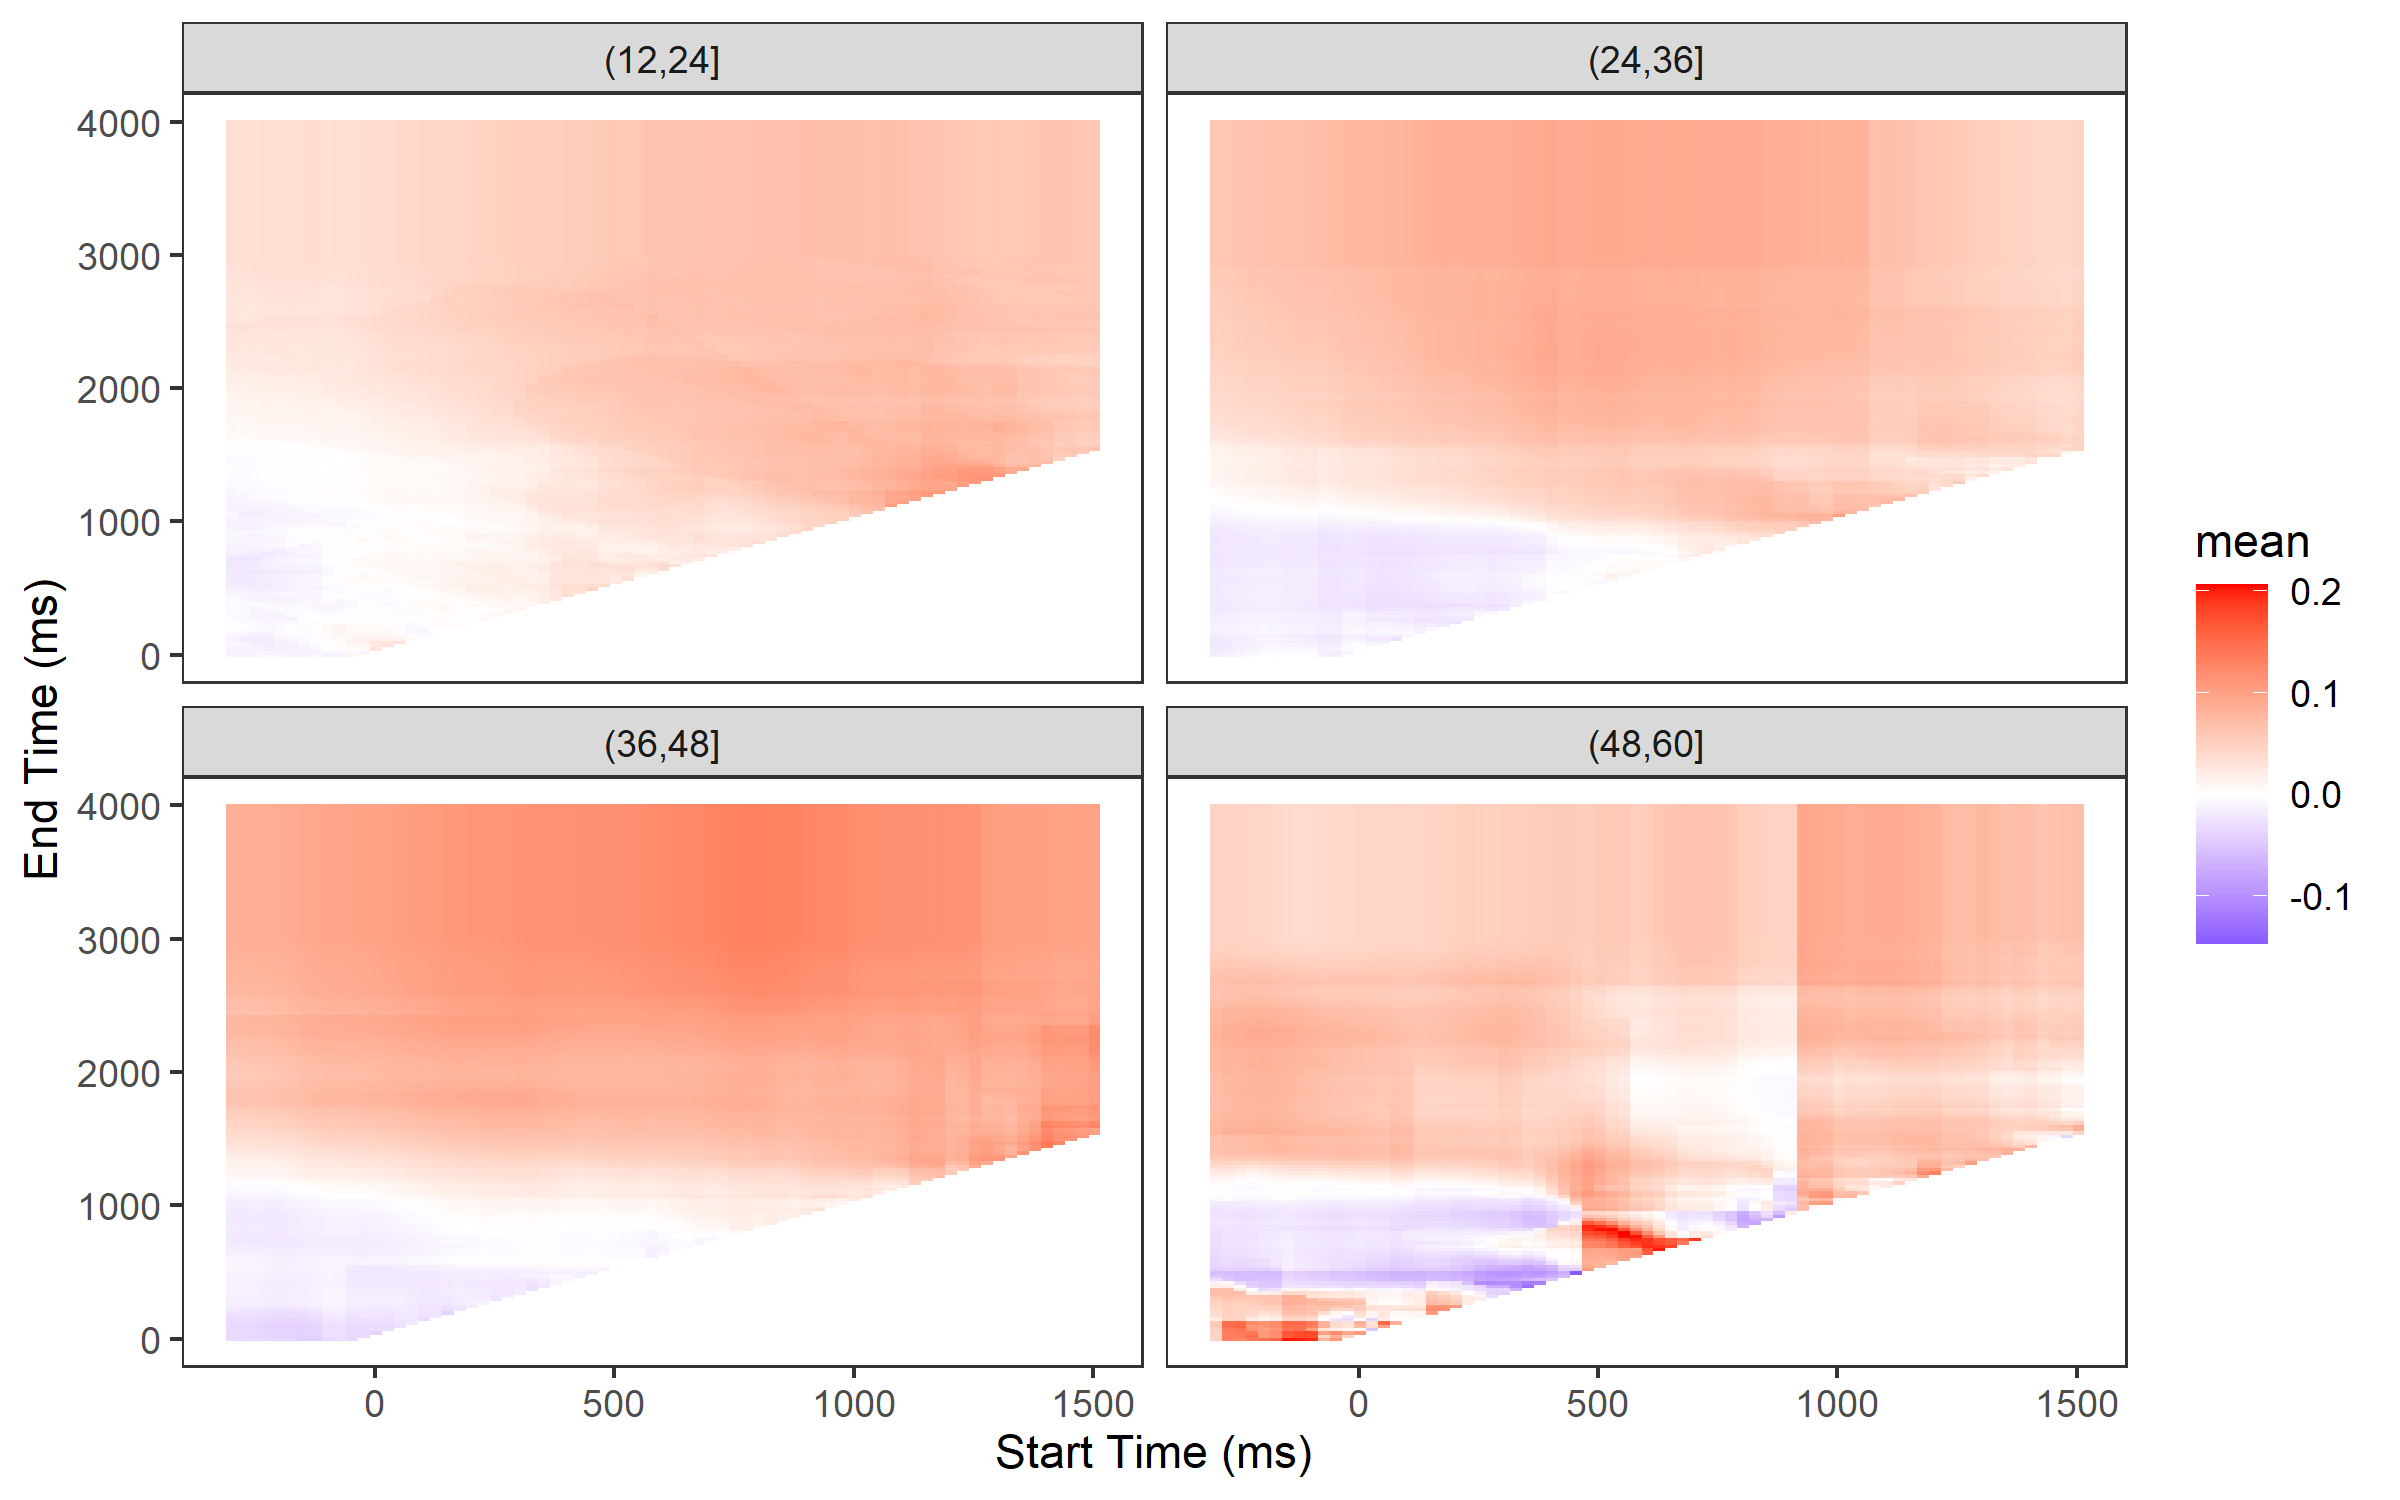
\includegraphics[width=13.6cm,height=8.5cm]{../figures/interitem_cors_window_analysis.png}
\caption{Participants' average inter-item correlation for proportion of looking time to familiar targets, as a function of window start time and end time, with each facet showing a different age group. More positive (red) correlations are more desirable, and blue/white represent start/end time combinations that researchers should avoid. Black lines highlight the region (start time: [300, 1000], end time: [2500, 4000]) in which IICs tend to be highest (mean = .093; range = [.042 - .131]).}
\label{fig:time_window}
\end{SCfigure*}

\hypertarget{discussion}{%
\section{Discussion}\label{discussion}}

Theoretical progress in understanding child development requires rich
datasets, but collecting child data is expensive, difficult, and
time-intensive. Recent years have seen a growing effort to build open
source tools and pool research efforts to meet the challenge of building
a cumulative developmental science (Bergmann et al., 2018; Frank,
Braginsky, Yurovsky, \& Marchman, 2017; The ManyBabies Consortium,
2020). The Peekbank project expands on these efforts by building an
infrastructure for aggregating eye-tracking data across studies, with a
specific focus on the looking-while-listening paradigm. The goals of the
database are to ask theory-driven questions about the development of
word knowledge and to establish methodological best-practices in infant
eye-tracking methods. This paper presents an illustration of some of the
key theoretical and methodological questions that can be addressed using
Peekbank: generalizing across item-level variability in children's word
recognition and providing data-driven guidance on choosing windows of
analysis.

Our first analysis shows that Peekbank can be used to model
item-independent changes in the speed and accuracy of word recognition
across development. Children showed age-related increases in the speed
of word recognition across one to five years of age, extending past
foundational work (e.g., Fernald et al., 1998) by showing that these
word processing gains generalize across items and are not only
attributable to word-specific gains in processing speed. Our second
analysis demonstrates how Peekbank can be used to make data-driven
analytic decisions, focusing on the choice of time windows for analysis.
In looking-while-listening studies, researchers often choose a
relatively short time window of roughly 300-1800 or 2000ms (Fernald et
al., 2008), with the justification that eye movements occurring after
this window may no longer be related to the target label (Swingley \&
Aslin, 2000). Our results suggest that researchers could consider
increasing the size of the time window for analyzing target fixations,
at least for familiar words, if their goal is to maximize consistent
signal in children's target fixations.

There are a number of limitations surrounding the current scope of the
database. A priority in future work will be to expand the size of the
database. With 15 datasets currently available, idiosyncrasies of
particular designs and condition manipulations still have substantial
influence on modeling results. Increasing the set of distinct datasets
will lead to more robust generalizations across item-level variability.
The current database is also limited by the relatively homogeneous
background of its participants, both with respect to language (mostly
monolingual native English speakers) and cultural background (all but
one dataset comes from WEIRD populations; Muthukrishna et al., 2020).
Broadening the diversity of participant backgrounds will expand the
scope of the generalizations we can form about child word recognition.

Finally, while the current database is focused on studies of word
recognition, the tools and infrastructure developed in the project can
in principle be used to accommodate any eye-tracking paradigm, opening
up new avenues for insights into cognitive development. Gaze behavior
has been at the core of many of the key advances in our understanding of
infant cognition. Aggregating large datasets of infant looking behavior
in a unified, openly-accessible format promises to bring a fuller
picture of infant cognitive development into view.

\hypertarget{acknowledgements}{%
\section{Acknowledgements}\label{acknowledgements}}

We would like to thank the labs and researchers that have made their
data publicly available in the database.

\hypertarget{references}{%
\section{References}\label{references}}

\setlength{\parindent}{-0.1in} 
\setlength{\leftskip}{0.125in}

\noindent

\hypertarget{refs}{}
\leavevmode\hypertarget{ref-Adams2018}{}%
Adams, K. A., Marchman, V. A., Loi, E. C., Ashland, M. D., Fernald, A.,
\& Feldman, H. M. (2018). Caregiver talk and medical risk as predictors
of language outcomes in full term and preterm toddlers. \emph{Child
Development}, \emph{89}(5), 1674--1690.

\leavevmode\hypertarget{ref-Bergelson2012a}{}%
Bergelson, E., \& Swingley, D. (2012). At 6-9 months, human infants know
the meanings of many common nouns. \emph{PNAS}, \emph{109}(9),
3253--3258.

\leavevmode\hypertarget{ref-Bergmann2018}{}%
Bergmann, C., Tsuji, S., Piccinini, P. E., Lewis, M. L., Braginsky, M.,
Frank, M. C., \& Cristia, A. (2018). Promoting replicability in
developmental research through meta-analyses: Insights from language
acquisition research. \emph{Child Development}, \emph{89}(6),
1996--2009.

\leavevmode\hypertarget{ref-Byers-Heinlein2017}{}%
Byers-Heinlein, K., Morin-Lessard, E., \& Lew-Williams, C. (2017).
Bilingual infants control their languages as they listen. \emph{PNAS},
201703220.

\leavevmode\hypertarget{ref-Casillas2017}{}%
Casillas, M., Brown, P., \& Levinson, S. (2017). Casillas HomeBank
Corpus. \url{http://doi.org/10.21415/T51X12}

\leavevmode\hypertarget{ref-Csibra2016}{}%
Csibra, G., Hernik, M., Mascaro, O., Tatone, D., \& Lengyel, M. (2016).
Statistical treatment of looking-time data. \emph{Developmental
Psychology}, \emph{52}(4), 521--536.

\leavevmode\hypertarget{ref-de-boeck2011}{}%
De Boeck, P., Bakker, M., Zwitser, R., Nivard, M., Hofman, A.,
Tuerlinckx, F., \& Partchev, I. (2011). The estimation of item response
models with the lmer function from the lme4 package in R. \emph{Journal
of Statistical Software}, \emph{39}(12), 1--28.

\leavevmode\hypertarget{ref-embretson2000}{}%
Embretson, S. E., \& Reise, S. P. (2000). \emph{Item response theory for
psychologists}. Mahwah, NJ: Lawrence Erlbaum.

\leavevmode\hypertarget{ref-Fernald2012a}{}%
Fernald, A., \& Marchman, V. A. (2012). Individual differences in
lexical processing at 18 months predict vocabulary growth in typically
developing and late-talking toddlers. \emph{Child Development},
\emph{83}(1), 203--22.

\leavevmode\hypertarget{ref-fernald1998}{}%
Fernald, A., Pinto, J. P., Swingley, D., Weinberg, A., \& McRoberts, G.
W. (1998). Rapid gains in speed of verbal processing by infants in the
2nd year. \emph{Psychological Science}, \emph{9}(3), 228--231.

\leavevmode\hypertarget{ref-Fernald2008}{}%
Fernald, A., Zangl, R., Portillo, A. L., \& Marchman, V. A. (2008).
Looking while listening: Using eye movements to monitor spoken language
comprehension by infants and young children. In I. A. Sekerina, E. M.
Fernandez, \& H. Clahsen (Eds.), \emph{Developmental psycholinguistics:
On-line methods in children's language processing} (pp. 97--135).
Amsterdam: John Benjamins.

\leavevmode\hypertarget{ref-Frank2016}{}%
Frank, M. C., Braginsky, M., Yurovsky, D., \& Marchman, V. A. (2017).
Wordbank: An open repository for developmental vocabulary data.
\emph{Journal of Child Language}, \emph{44}(3), 677--694.

\leavevmode\hypertarget{ref-frank2021}{}%
Frank, M. C., Braginsky, M., Yurovsky, D., \& Marchman, V. A. (2021).
\emph{Variability and Consistency in Early Language Learning: The
Wordbank Project}. Cambridge, MA: MIT Press.

\leavevmode\hypertarget{ref-frank2016b}{}%
Frank, M. C., Lewis, M., \& MacDonald, K. (2016). A performance model
for early word learning. In \emph{Proceedings of the 38th Annual
Conference of the Cognitive Science Society} (pp. 2610--2614). Austin,
TX: Cognitive Science Society.

\leavevmode\hypertarget{ref-Garrison2020}{}%
Garrison, H., Baudet, G., Breitfeld, E., Aberman, A., \& Bergelson, E.
(2020). Familiarity plays a small role in noun comprehension at 12--18
months. \emph{Infancy}, \emph{25}(4), 458--477.

\leavevmode\hypertarget{ref-Golinkoff2013}{}%
Golinkoff, R. M., Ma, W., Song, L., \& Hirsh-Pasek, K. (2013).
Twenty-five years using the intermodal preferential looking paradigm to
study language acquisition: What have we learned? \emph{Perspectives on
Psychol. Science}, \emph{8}(3), 316--339.

\leavevmode\hypertarget{ref-Hirsh-Pasek1987}{}%
Hirsh-Pasek, K., Cauley, K. M., Golinkoff, R. M., \& Gordon, L. (1987).
The eyes have it: Lexical and syntactic comprehension in a new paradigm.
\emph{Journal of Child Language}, \emph{14}(1), 23--45.

\leavevmode\hypertarget{ref-Huang2020}{}%
Huang, Y., \& Snedeker, J. (2020). Evidence from the visual world
paradigm raises questions about unaccusativity and growth curve
analyses. \emph{Cognition}, \emph{200}, 104251.

\leavevmode\hypertarget{ref-kail1991}{}%
Kail, R. (1991). Developmental change in speed of processing during
childhood and adolescence. \emph{Psychological Bulletin}, \emph{109}(3),
490.

\leavevmode\hypertarget{ref-Lew-Williams2007}{}%
Lew-Williams, C., \& Fernald, A. (2007). Young children learning Spanish
make rapid use of grammatical gender in spoken word recognition.
\emph{Psychological Science}, \emph{18}(3), 193--198.

\leavevmode\hypertarget{ref-Mahr2015}{}%
Mahr, T., McMillan, B. T. M., Saffran, J. R., Ellis Weismer, S., \&
Edwards, J. (2015). Anticipatory coarticulation facilitates word
recognition in toddlers. \emph{Cognition}, \emph{142}, 345--350.

\leavevmode\hypertarget{ref-Marchman2008}{}%
Marchman, V. A., \& Fernald, A. (2008). Speed of word recognition and
vocabulary knowledge in infancy predict cognitive and language outcomes
in later childhood. \emph{Developmental Science}, \emph{11}(3), F9--16.

\leavevmode\hypertarget{ref-Marchman2018}{}%
Marchman, V. A., Loi, E. C., Adams, K. A., Ashland, M., Fernald, A., \&
Feldman, H. M. (2018). Speed of language comprehension at 18 months old
predicts school-relevant outcomes at 54 months old in children born
preterm. \emph{Journal of Developmental and Behavioral Pediatrics},
\emph{39}(3), 246--253.

\leavevmode\hypertarget{ref-Mirman2014}{}%
Mirman, D. (2014). \emph{Growth curve analysis and visualization using
R}. Boca Raton, FL: CRC Press.

\leavevmode\hypertarget{ref-Muthukrishna2020}{}%
Muthukrishna, M., Bell, A. V., Henrich, J., Curtin, C. M., Gedranovich,
A., McInerney, J., \& Thue, B. (2020). Beyond Western, educated,
industrial, rich, and democratic (WEIRD) psychology: Measuring and
mapping scales of cultural and psychological distance.
\emph{Psychological Science}, \emph{31}(6), 678--701.

\leavevmode\hypertarget{ref-Peelle2020}{}%
Peelle, J. E., \& Van Engen, K. J. (2020). Time stand still: Effects of
temporal window selection on eye tracking analysis. \emph{PsyArXiv}.
\url{http://doi.org/https://doi.org/10.31234/osf.io/pc3da}

\leavevmode\hypertarget{ref-Perry2017}{}%
Perry, L. K., \& Saffran, J. R. (2017). Is a pink cow still a cow?
Individual differences in toddlers' vocabulary knowledge and lexical
representations. \emph{Cognitive Science}, \emph{41}(4), 1090--1105.
\url{http://doi.org/10.1111/cogs.12370}

\leavevmode\hypertarget{ref-peter2019}{}%
Peter, M. S., Durrant, S., Jessop, A., Bidgood, A., Pine, J. M., \&
Rowland, C. F. (2019). Does speed of processing or vocabulary size
predict later language growth in toddlers? \emph{Cognitive Psychology},
\emph{115}, 101238.

\leavevmode\hypertarget{ref-Pomper2016}{}%
Pomper, R., \& Saffran, J. R. (2016). Roses are red, socks are blue:
Switching dimensions disrupts young children's language comprehension.
\emph{Plos One}, \emph{11}(6), e0158459.

\leavevmode\hypertarget{ref-Pomper2019}{}%
Pomper, R., \& Saffran, J. R. (2019). Familiar object salience affects
novel word learning. \emph{Child Development}, \emph{90}(2), e246--e262.

\leavevmode\hypertarget{ref-Potter2019}{}%
Potter, C. E., Fourakis, E., Morin-Lessard, E., Byers-Heinlein, K., \&
Lew-Williams, C. (2019). Bilingual toddlers' comprehension of mixed
sentences is asymmetrical across their two languages.
\emph{Developmental Science}, \emph{22}(4), 1--9.

\leavevmode\hypertarget{ref-RDevelopmentCoreTeam2010}{}%
R Development Core Team. (2020). R: A language and environment for
statistical computing. Vienna, Austria: R Foundation for Statistical
Computing.

\leavevmode\hypertarget{ref-steegenEtAl2016}{}%
Steegen, S., Tuerlinckx, F., Gelman, A., \& Vanpaemel, W. (2016).
Increasing transparency through a multiverse analysis.
\emph{Perspectives on Psychol. Science}, \emph{11}(5), 702--712.

\leavevmode\hypertarget{ref-Swingley2000}{}%
Swingley, D., \& Aslin, R. N. (2000). Spoken word recognition and
lexical representation in very young children. \emph{Cognition},
\emph{76}(2), 147--66.

\leavevmode\hypertarget{ref-Swingley2002}{}%
Swingley, D., \& Aslin, R. N. (2002). Lexical neighborhoods and the
word-form representations of 14-month-olds. \emph{Psychological
Science}, \emph{13}(5), 480--484.

\leavevmode\hypertarget{ref-TheManyBabiesConsortium2020}{}%
The ManyBabies Consortium. (2020). Quantifying sources of variability in
infancy research using the infant-directed speech preference.
\emph{Advances in Methods and Practices in Psychological Science},
\emph{3}(1), 24--52.

\leavevmode\hypertarget{ref-Wickham2019}{}%
Wickham, H., Averick, M., Bryan, J., Chang, W., McGowan, L. D.,
François, R., \ldots{} Yutani, H. (2019). Welcome to the tidyverse.
\emph{Journal of Open Source Software}, \emph{4}(43), 1686.

\leavevmode\hypertarget{ref-Yurovsky2017}{}%
Yurovsky, D., \& Frank, M. C. (2017). Beyond naïve cue combination:
Salience and social cues in early word learning. \emph{Developmental
Science}, \emph{20}(2), 1--17.

\leavevmode\hypertarget{ref-Yurovsky2013}{}%
Yurovsky, D., Wade, A., \& Frank, M. C. (2013). Online processing of
speech and social information in early word learning. In
\emph{Proceedings of the 35th Annual Conference of the Cognitive Science
Society} (pp. 1641--1646). Austin, TX: Cognitive Science Society.

\bibliographystyle{apacite}


\end{document}
